\documentclass[1p]{elsarticle_modified}
%\bibliographystyle{elsarticle-num}

%\usepackage[colorlinks]{hyperref}
%\usepackage{abbrmath_seonhwa} %\Abb, \Ascr, \Acal ,\Abf, \Afrak
\usepackage{amsfonts}
\usepackage{amssymb}
\usepackage{amsmath}
\usepackage{amsthm}
\usepackage{scalefnt}
\usepackage{amsbsy}
\usepackage{kotex}
\usepackage{caption}
\usepackage{subfig}
\usepackage{color}
\usepackage{graphicx}
\usepackage{xcolor} %% white, black, red, green, blue, cyan, magenta, yellow
\usepackage{float}
\usepackage{setspace}
\usepackage{hyperref}

\usepackage{tikz}
\usetikzlibrary{arrows}

\usepackage{multirow}
\usepackage{array} % fixed length table
\usepackage{hhline}

%%%%%%%%%%%%%%%%%%%%%
\makeatletter
\renewcommand*\env@matrix[1][\arraystretch]{%
	\edef\arraystretch{#1}%
	\hskip -\arraycolsep
	\let\@ifnextchar\new@ifnextchar
	\array{*\c@MaxMatrixCols c}}
\makeatother %https://tex.stackexchange.com/questions/14071/how-can-i-increase-the-line-spacing-in-a-matrix
%%%%%%%%%%%%%%%

\usepackage[normalem]{ulem}

\newcommand{\msout}[1]{\ifmmode\text{\sout{\ensuremath{#1}}}\else\sout{#1}\fi}
%SOURCE: \msout is \stkout macro in https://tex.stackexchange.com/questions/20609/strikeout-in-math-mode

\newcommand{\cancel}[1]{
	\ifmmode
	{\color{red}\msout{#1}}
	\else
	{\color{red}\sout{#1}}
	\fi
}

\newcommand{\add}[1]{
	{\color{blue}\uwave{#1}}
}

\newcommand{\replace}[2]{
	\ifmmode
	{\color{red}\msout{#1}}{\color{blue}\uwave{#2}}
	\else
	{\color{red}\sout{#1}}{\color{blue}\uwave{#2}}
	\fi
}

\newcommand{\Sol}{\mathcal{S}} %segment
\newcommand{\D}{D} %diagram
\newcommand{\A}{\mathcal{A}} %arc


%%%%%%%%%%%%%%%%%%%%%%%%%%%%%5 test

\def\sl{\operatorname{\textup{SL}}(2,\Cbb)}
\def\psl{\operatorname{\textup{PSL}}(2,\Cbb)}
\def\quan{\mkern 1mu \triangleright \mkern 1mu}

\theoremstyle{definition}
\newtheorem{thm}{Theorem}[section]
\newtheorem{prop}[thm]{Proposition}
\newtheorem{lem}[thm]{Lemma}
\newtheorem{ques}[thm]{Question}
\newtheorem{cor}[thm]{Corollary}
\newtheorem{defn}[thm]{Definition}
\newtheorem{exam}[thm]{Example}
\newtheorem{rmk}[thm]{Remark}
\newtheorem{alg}[thm]{Algorithm}

\newcommand{\I}{\sqrt{-1}}
\begin{document}

%\begin{frontmatter}
%
%\title{Boundary parabolic representations of knots up to 8 crossings}
%
%%% Group authors per affiliation:
%\author{Yunhi Cho} 
%\address{Department of Mathematics, University of Seoul, Seoul, Korea}
%\ead{yhcho@uos.ac.kr}
%
%
%\author{Seonhwa Kim} %\fnref{s_kim}}
%\address{Center for Geometry and Physics, Institute for Basic Science, Pohang, 37673, Korea}
%\ead{ryeona17@ibs.re.kr}
%
%\author{Hyuk Kim}
%\address{Department of Mathematical Sciences, Seoul National University, Seoul 08826, Korea}
%\ead{hyukkim@snu.ac.kr}
%
%\author{Seokbeom Yoon}
%\address{Department of Mathematical Sciences, Seoul National University, Seoul, 08826,  Korea}
%\ead{sbyoon15@snu.ac.kr}
%
%\begin{abstract}
%We find all boundary parabolic representation of knots up to 8 crossings.
%
%\end{abstract}
%\begin{keyword}
%    \MSC[2010] 57M25 
%\end{keyword}
%
%\end{frontmatter}

%\linenumbers
%\tableofcontents
%
\newcommand\colored[1]{\textcolor{white}{\rule[-0.35ex]{0.8em}{1.4ex}}\kern-0.8em\color{red} #1}%
%\newcommand\colored[1]{\textcolor{white}{ #1}\kern-2.17ex	\textcolor{white}{ #1}\kern-1.81ex	\textcolor{white}{ #1}\kern-2.15ex\color{red}#1	}

{\Large $\underline{12a_{0129}~(K12a_{0129})}$}

\setlength{\tabcolsep}{10pt}
\renewcommand{\arraystretch}{1.6}
\vspace{1cm}\begin{tabular}{m{100pt}>{\centering\arraybackslash}m{274pt}}
\multirow{5}{120pt}{
	\centering
	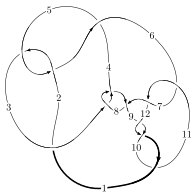
\includegraphics[width=112pt]{../../../GIT/diagram.site/Diagrams/png/930_12a_0129.png}\\
\ \ \ A knot diagram\footnotemark}&
\allowdisplaybreaks
\textbf{Linearized knot diagam} \\
\cline{2-2}
 &
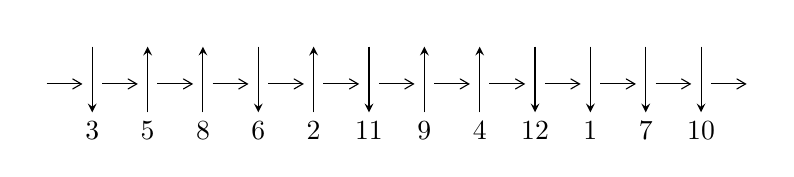
\begin{tikzpicture}[x=20pt, y=17pt]
	% nodes
	\node (C0) at (0, 0) {};
	\node (C1) at (1, 0) {};
	\node (C1U) at (1, +1) {};
	\node (C1D) at (1, -1) {3};

	\node (C2) at (2, 0) {};
	\node (C2U) at (2, +1) {};
	\node (C2D) at (2, -1) {5};

	\node (C3) at (3, 0) {};
	\node (C3U) at (3, +1) {};
	\node (C3D) at (3, -1) {8};

	\node (C4) at (4, 0) {};
	\node (C4U) at (4, +1) {};
	\node (C4D) at (4, -1) {6};

	\node (C5) at (5, 0) {};
	\node (C5U) at (5, +1) {};
	\node (C5D) at (5, -1) {2};

	\node (C6) at (6, 0) {};
	\node (C6U) at (6, +1) {};
	\node (C6D) at (6, -1) {11};

	\node (C7) at (7, 0) {};
	\node (C7U) at (7, +1) {};
	\node (C7D) at (7, -1) {9};

	\node (C8) at (8, 0) {};
	\node (C8U) at (8, +1) {};
	\node (C8D) at (8, -1) {4};

	\node (C9) at (9, 0) {};
	\node (C9U) at (9, +1) {};
	\node (C9D) at (9, -1) {12};

	\node (C10) at (10, 0) {};
	\node (C10U) at (10, +1) {};
	\node (C10D) at (10, -1) {1};

	\node (C11) at (11, 0) {};
	\node (C11U) at (11, +1) {};
	\node (C11D) at (11, -1) {7};

	\node (C12) at (12, 0) {};
	\node (C12U) at (12, +1) {};
	\node (C12D) at (12, -1) {10};
	\node (C13) at (13, 0) {};

	% arrows
	\draw[->,>={angle 60}]
	(C0) edge (C1) (C1) edge (C2) (C2) edge (C3) (C3) edge (C4) (C4) edge (C5) (C5) edge (C6) (C6) edge (C7) (C7) edge (C8) (C8) edge (C9) (C9) edge (C10) (C10) edge (C11) (C11) edge (C12) (C12) edge (C13) ;	\draw[->,>=stealth]
	(C1U) edge (C1D) (C2D) edge (C2U) (C3D) edge (C3U) (C4U) edge (C4D) (C5D) edge (C5U) (C6U) edge (C6D) (C7D) edge (C7U) (C8D) edge (C8U) (C9U) edge (C9D) (C10U) edge (C10D) (C11U) edge (C11D) (C12U) edge (C12D) ;
	\end{tikzpicture} \\
\hhline{~~} \\& 
\textbf{Solving Sequence} \\ \cline{2-2} 
 &
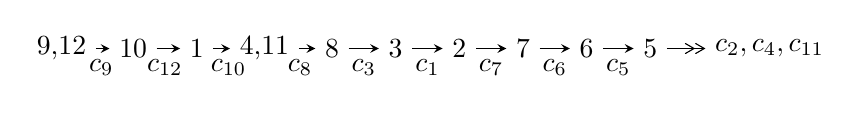
\begin{tikzpicture}[x=23pt, y=7pt]
	% node
	\node (A0) at (-1/8, 0) {9,12};
	\node (A1) at (1, 0) {10};
	\node (A2) at (2, 0) {1};
	\node (A3) at (49/16, 0) {4,11};
	\node (A4) at (33/8, 0) {8};
	\node (A5) at (41/8, 0) {3};
	\node (A6) at (49/8, 0) {2};
	\node (A7) at (57/8, 0) {7};
	\node (A8) at (65/8, 0) {6};
	\node (A9) at (73/8, 0) {5};
	\node (C1) at (1/2, -1) {$c_{9}$};
	\node (C2) at (3/2, -1) {$c_{12}$};
	\node (C3) at (5/2, -1) {$c_{10}$};
	\node (C4) at (29/8, -1) {$c_{8}$};
	\node (C5) at (37/8, -1) {$c_{3}$};
	\node (C6) at (45/8, -1) {$c_{1}$};
	\node (C7) at (53/8, -1) {$c_{7}$};
	\node (C8) at (61/8, -1) {$c_{6}$};
	\node (C9) at (69/8, -1) {$c_{5}$};
	\node (A10) at (11, 0) {$c_{2},c_{4},c_{11}$};

	% edge
	\draw[->,>=stealth]	
	(A0) edge (A1) (A1) edge (A2) (A2) edge (A3) (A3) edge (A4) (A4) edge (A5) (A5) edge (A6) (A6) edge (A7) (A7) edge (A8) (A8) edge (A9) ;
	\draw[->>,>={angle 60}]	
	(A9) edge (A10);
\end{tikzpicture} \\ 

\end{tabular} \\

\footnotetext{
The image of knot diagram is generated by the software ``\textbf{Draw programme}" developed by Andrew Bartholomew(\url{http://www.layer8.co.uk/maths/draw/index.htm\#Running-draw}), where we modified some parts for our purpose(\url{https://github.com/CATsTAILs/LinksPainter}).
}\phantom \\ \newline 
\centering \textbf{Ideals for irreducible components\footnotemark of $X_{\text{par}}$} 
 
\begin{align*}
I^u_{1}&=\langle 
-4.61547\times10^{58} u^{89}-4.83832\times10^{59} u^{88}+\cdots+1.64419\times10^{56} b+2.98980\times10^{58},\\
\phantom{I^u_{1}}&\phantom{= \langle  }-6.46398\times10^{59} u^{89}-6.85486\times10^{60} u^{88}+\cdots+1.64419\times10^{56} a+4.63218\times10^{59},\\
\phantom{I^u_{1}}&\phantom{= \langle  }u^{90}+12 u^{89}+\cdots-6 u-1\rangle \\
I^u_{2}&=\langle 
3 a^8+31 a^7+13 a^6+178 a^5+16 a^4+212 a^3-28 a^2+61 b+39 a-18,\\
\phantom{I^u_{2}}&\phantom{= \langle  }a^9+6 a^7+a^6+9 a^5+2 a^4+6 a^3+a^2+2 a+1,\;u-1\rangle \\
I^u_{3}&=\langle 
b,\;a^2+a u+2 a+3 u+5,\;u^2+u-1\rangle \\
\\
\end{align*}
\raggedright * 3 irreducible components of $\dim_{\mathbb{C}}=0$, with total 103 representations.\\
\footnotetext{All coefficients of polynomials are rational numbers. But the coefficients are sometimes approximated in decimal forms when there is not enough margin.}
\newpage
\renewcommand{\arraystretch}{1}
\centering \section*{I. $I^u_{1}= \langle -4.62\times10^{58} u^{89}-4.84\times10^{59} u^{88}+\cdots+1.64\times10^{56} b+2.99\times10^{58},\;-6.46\times10^{59} u^{89}-6.85\times10^{60} u^{88}+\cdots+1.64\times10^{56} a+4.63\times10^{59},\;u^{90}+12 u^{89}+\cdots-6 u-1 \rangle$}
\flushleft \textbf{(i) Arc colorings}\\
\begin{tabular}{m{7pt} m{180pt} m{7pt} m{180pt} }
\flushright $a_{9}=$&$\begin{pmatrix}1\\0\end{pmatrix}$ \\
\flushright $a_{12}=$&$\begin{pmatrix}0\\u\end{pmatrix}$ \\
\flushright $a_{10}=$&$\begin{pmatrix}1\\u^2\end{pmatrix}$ \\
\flushright $a_{1}=$&$\begin{pmatrix}- u\\- u^3+u\end{pmatrix}$ \\
\flushright $a_{4}=$&$\begin{pmatrix}3931.41 u^{89}+41691.5 u^{88}+\cdots-14878.3 u-2817.31\\280.715 u^{89}+2942.68 u^{88}+\cdots-973.725 u-181.840\end{pmatrix}$ \\
\flushright $a_{11}=$&$\begin{pmatrix}- u^2+1\\- u^4+2 u^2\end{pmatrix}$ \\
\flushright $a_{8}=$&$\begin{pmatrix}-2618.93 u^{89}-27889.5 u^{88}+\cdots+10177.0 u+1934.72\\-5355.91 u^{89}-57017.6 u^{88}+\cdots+20797.5 u+3951.82\end{pmatrix}$ \\
\flushright $a_{3}=$&$\begin{pmatrix}6611.43 u^{89}+70073.2 u^{88}+\cdots-24950.5 u-4721.38\\7255.63 u^{89}+76897.0 u^{88}+\cdots-27351.2 u-5173.98\end{pmatrix}$ \\
\flushright $a_{2}=$&$\begin{pmatrix}-5522.62 u^{89}-58631.2 u^{88}+\cdots+21058.6 u+3993.67\\-8007.18 u^{89}-85082.8 u^{88}+\cdots+30711.5 u+5824.77\end{pmatrix}$ \\
\flushright $a_{7}=$&$\begin{pmatrix}2736.97 u^{89}+29128.0 u^{88}+\cdots-10620.5 u-2017.09\\-5355.91 u^{89}-57017.6 u^{88}+\cdots+20797.5 u+3951.82\end{pmatrix}$ \\
\flushright $a_{6}=$&$\begin{pmatrix}-414.169 u^{89}-4382.73 u^{88}+\cdots+1550.44 u+294.488\\-4375.24 u^{89}-46535.3 u^{88}+\cdots+16888.5 u+3206.23\end{pmatrix}$ \\
\flushright $a_{5}=$&$\begin{pmatrix}5357.29 u^{89}+56777.6 u^{88}+\cdots-20209.9 u-3823.63\\5572.68 u^{89}+59009.0 u^{88}+\cdots-20877.5 u-3945.62\end{pmatrix}$\\&\end{tabular}
\flushleft \textbf{(ii) Obstruction class $= -1$}\\~\\
\flushleft \textbf{(iii) Cusp Shapes $= -11889.9 u^{89}-126101. u^{88}+\cdots+45065.9 u+8536.51$}\\~\\
\newpage\renewcommand{\arraystretch}{1}
\flushleft \textbf{(iv) u-Polynomials at the component}\newline \\
\begin{tabular}{m{50pt}|m{274pt}}
Crossings & \hspace{64pt}u-Polynomials at each crossing \\
\hline $$\begin{aligned}c_{1},c_{4}\end{aligned}$$&$\begin{aligned}
&u^{90}+32 u^{89}+\cdots-34 u+1
\end{aligned}$\\
\hline $$\begin{aligned}c_{2},c_{5}\end{aligned}$$&$\begin{aligned}
&u^{90}+4 u^{89}+\cdots-10 u+1
\end{aligned}$\\
\hline $$\begin{aligned}c_{3},c_{8}\end{aligned}$$&$\begin{aligned}
&u^{90}-2 u^{89}+\cdots-80 u-16
\end{aligned}$\\
\hline $$\begin{aligned}c_{6},c_{11}\end{aligned}$$&$\begin{aligned}
&u^{90}+3 u^{89}+\cdots+1024 u+512
\end{aligned}$\\
\hline $$\begin{aligned}c_{7}\end{aligned}$$&$\begin{aligned}
&u^{90}-30 u^{89}+\cdots-3712 u+256
\end{aligned}$\\
\hline $$\begin{aligned}c_{9},c_{10},c_{12}\end{aligned}$$&$\begin{aligned}
&u^{90}-12 u^{89}+\cdots+6 u-1
\end{aligned}$\\
\hline
\end{tabular}\\~\\
\newpage\renewcommand{\arraystretch}{1}
\flushleft \textbf{(v) Riley Polynomials at the component}\newline \\
\begin{tabular}{m{50pt}|m{274pt}}
Crossings & \hspace{64pt}Riley Polynomials at each crossing \\
\hline $$\begin{aligned}c_{1},c_{4}\end{aligned}$$&$\begin{aligned}
&y^{90}+56 y^{89}+\cdots-3090 y+1
\end{aligned}$\\
\hline $$\begin{aligned}c_{2},c_{5}\end{aligned}$$&$\begin{aligned}
&y^{90}+32 y^{89}+\cdots-34 y+1
\end{aligned}$\\
\hline $$\begin{aligned}c_{3},c_{8}\end{aligned}$$&$\begin{aligned}
&y^{90}-30 y^{89}+\cdots-3712 y+256
\end{aligned}$\\
\hline $$\begin{aligned}c_{6},c_{11}\end{aligned}$$&$\begin{aligned}
&y^{90}-63 y^{89}+\cdots-4194304 y+262144
\end{aligned}$\\
\hline $$\begin{aligned}c_{7}\end{aligned}$$&$\begin{aligned}
&y^{90}+54 y^{89}+\cdots-4923392 y+65536
\end{aligned}$\\
\hline $$\begin{aligned}c_{9},c_{10},c_{12}\end{aligned}$$&$\begin{aligned}
&y^{90}-92 y^{89}+\cdots+22 y+1
\end{aligned}$\\
\hline
\end{tabular}\\~\\
\newpage\flushleft \textbf{(vi) Complex Volumes and Cusp Shapes}
$$\begin{array}{c|c|c}  
\text{Solutions to }I^u_{1}& \I (\text{vol} + \sqrt{-1}CS) & \text{Cusp shape}\\
 \hline 
\begin{aligned}
u &= \phantom{-}0.636017 + 0.771523 I \\
a &= \phantom{-}0.189507 + 0.291046 I \\
b &= \phantom{-}0.809550 + 0.779235 I\end{aligned}
 & -6.14252 + 0.17816 I & \phantom{-0.000000 } 0 \\ \hline\begin{aligned}
u &= \phantom{-}0.636017 - 0.771523 I \\
a &= \phantom{-}0.189507 - 0.291046 I \\
b &= \phantom{-}0.809550 - 0.779235 I\end{aligned}
 & -6.14252 - 0.17816 I & \phantom{-0.000000 } 0 \\ \hline\begin{aligned}
u &= \phantom{-}0.432828 + 0.882468 I \\
a &= \phantom{-}0.666021 + 0.933229 I \\
b &= -1.044510 + 0.696314 I\end{aligned}
 & \phantom{-}0.35982 - 6.42463 I & \phantom{-0.000000 } 0 \\ \hline\begin{aligned}
u &= \phantom{-}0.432828 - 0.882468 I \\
a &= \phantom{-}0.666021 - 0.933229 I \\
b &= -1.044510 - 0.696314 I\end{aligned}
 & \phantom{-}0.35982 + 6.42463 I & \phantom{-0.000000 } 0 \\ \hline\begin{aligned}
u &= \phantom{-}0.518572 + 0.830971 I \\
a &= -0.817139 - 1.151630 I \\
b &= \phantom{-}0.929384 - 0.742004 I\end{aligned}
 & -5.77013 - 5.56186 I & \phantom{-0.000000 } 0 \\ \hline\begin{aligned}
u &= \phantom{-}0.518572 - 0.830971 I \\
a &= -0.817139 + 1.151630 I \\
b &= \phantom{-}0.929384 + 0.742004 I\end{aligned}
 & -5.77013 + 5.56186 I & \phantom{-0.000000 } 0 \\ \hline\begin{aligned}
u &= \phantom{-}0.456988 + 0.912736 I \\
a &= -0.595801 - 1.004760 I \\
b &= \phantom{-}1.056730 - 0.742766 I\end{aligned}
 & -0.93673 - 12.04190 I & \phantom{-0.000000 } 0 \\ \hline\begin{aligned}
u &= \phantom{-}0.456988 - 0.912736 I \\
a &= -0.595801 + 1.004760 I \\
b &= \phantom{-}1.056730 + 0.742766 I\end{aligned}
 & -0.93673 + 12.04190 I & \phantom{-0.000000 } 0 \\ \hline\begin{aligned}
u &= \phantom{-}0.780880 + 0.714283 I \\
a &= -0.311800 - 0.057546 I \\
b &= -0.901778 - 0.603260 I\end{aligned}
 & -0.709182 + 0.976820 I & \phantom{-0.000000 } 0 \\ \hline\begin{aligned}
u &= \phantom{-}0.780880 - 0.714283 I \\
a &= -0.311800 + 0.057546 I \\
b &= -0.901778 + 0.603260 I\end{aligned}
 & -0.709182 - 0.976820 I & \phantom{-0.000000 } 0\\
 \hline 
 \end{array}$$\newpage$$\begin{array}{c|c|c}  
\text{Solutions to }I^u_{1}& \I (\text{vol} + \sqrt{-1}CS) & \text{Cusp shape}\\
 \hline 
\begin{aligned}
u &= \phantom{-}0.936431 + 0.058571 I \\
a &= \phantom{-}0.16332 + 3.81110 I \\
b &= \phantom{-}0.031091 + 0.410222 I\end{aligned}
 & -1.33868 - 2.18003 I & \phantom{-0.000000 } 0 \\ \hline\begin{aligned}
u &= \phantom{-}0.936431 - 0.058571 I \\
a &= \phantom{-}0.16332 - 3.81110 I \\
b &= \phantom{-}0.031091 - 0.410222 I\end{aligned}
 & -1.33868 + 2.18003 I & \phantom{-0.000000 } 0 \\ \hline\begin{aligned}
u &= \phantom{-}0.481476 + 0.768915 I \\
a &= -0.015198 + 0.457099 I \\
b &= \phantom{-}0.658845 + 0.897569 I\end{aligned}
 & -2.16958 - 5.97918 I & \phantom{-0.000000 } 0 \\ \hline\begin{aligned}
u &= \phantom{-}0.481476 - 0.768915 I \\
a &= -0.015198 - 0.457099 I \\
b &= \phantom{-}0.658845 - 0.897569 I\end{aligned}
 & -2.16958 + 5.97918 I & \phantom{-0.000000 } 0 \\ \hline\begin{aligned}
u &= \phantom{-}0.776384 + 0.779070 I \\
a &= \phantom{-}0.378854 + 0.145892 I \\
b &= \phantom{-}0.952795 + 0.670266 I\end{aligned}
 & -1.90172 + 6.33365 I & \phantom{-0.000000 } 0 \\ \hline\begin{aligned}
u &= \phantom{-}0.776384 - 0.779070 I \\
a &= \phantom{-}0.378854 - 0.145892 I \\
b &= \phantom{-}0.952795 - 0.670266 I\end{aligned}
 & -1.90172 - 6.33365 I & \phantom{-0.000000 } 0 \\ \hline\begin{aligned}
u &= \phantom{-}0.569713 + 0.687366 I \\
a &= -1.21121 - 1.33527 I \\
b &= \phantom{-}0.752169 - 0.679210 I\end{aligned}
 & -2.52210 + 1.10076 I & \phantom{-0.000000 } 0 \\ \hline\begin{aligned}
u &= \phantom{-}0.569713 - 0.687366 I \\
a &= -1.21121 + 1.33527 I \\
b &= \phantom{-}0.752169 + 0.679210 I\end{aligned}
 & -2.52210 - 1.10076 I & \phantom{-0.000000 } 0 \\ \hline\begin{aligned}
u &= \phantom{-}0.457951 + 0.718324 I \\
a &= \phantom{-}1.14669 + 0.97490 I \\
b &= -0.867324 + 0.598381 I\end{aligned}
 & -0.83297 - 3.71434 I & \phantom{-0.000000 } 0 \\ \hline\begin{aligned}
u &= \phantom{-}0.457951 - 0.718324 I \\
a &= \phantom{-}1.14669 - 0.97490 I \\
b &= -0.867324 - 0.598381 I\end{aligned}
 & -0.83297 + 3.71434 I & \phantom{-0.000000 } 0\\
 \hline 
 \end{array}$$\newpage$$\begin{array}{c|c|c}  
\text{Solutions to }I^u_{1}& \I (\text{vol} + \sqrt{-1}CS) & \text{Cusp shape}\\
 \hline 
\begin{aligned}
u &= \phantom{-}0.478612 + 0.682084 I \\
a &= \phantom{-}0.114604 - 0.343684 I \\
b &= -0.590308 - 0.817882 I\end{aligned}
 & -0.975354 - 0.759900 I & \phantom{-0.000000 } 0 \\ \hline\begin{aligned}
u &= \phantom{-}0.478612 - 0.682084 I \\
a &= \phantom{-}0.114604 + 0.343684 I \\
b &= -0.590308 + 0.817882 I\end{aligned}
 & -0.975354 + 0.759900 I & \phantom{-0.000000 } 0 \\ \hline\begin{aligned}
u &= \phantom{-}1.167340 + 0.055219 I \\
a &= -0.02349 - 1.86427 I \\
b &= \phantom{-}0.552125 - 0.411305 I\end{aligned}
 & -2.59551 - 1.48754 I & \phantom{-0.000000 } 0 \\ \hline\begin{aligned}
u &= \phantom{-}1.167340 - 0.055219 I \\
a &= -0.02349 + 1.86427 I \\
b &= \phantom{-}0.552125 + 0.411305 I\end{aligned}
 & -2.59551 + 1.48754 I & \phantom{-0.000000 } 0 \\ \hline\begin{aligned}
u &= \phantom{-}0.812411\phantom{ +0.000000I} \\
a &= \phantom{-}0.583852\phantom{ +0.000000I} \\
b &= -0.370124\phantom{ +0.000000I}\end{aligned}
 & -1.14251\phantom{ +0.000000I} & \phantom{-0.000000 } 0 \\ \hline\begin{aligned}
u &= \phantom{-}1.150390 + 0.427470 I \\
a &= -0.448720 + 0.822247 I \\
b &= -0.981187 + 0.022086 I\end{aligned}
 & \phantom{-}1.90684 + 1.30777 I & \phantom{-0.000000 } 0 \\ \hline\begin{aligned}
u &= \phantom{-}1.150390 - 0.427470 I \\
a &= -0.448720 - 0.822247 I \\
b &= -0.981187 - 0.022086 I\end{aligned}
 & \phantom{-}1.90684 - 1.30777 I & \phantom{-0.000000 } 0 \\ \hline\begin{aligned}
u &= \phantom{-}1.210720 + 0.384439 I \\
a &= \phantom{-}0.497494 - 0.983806 I \\
b &= \phantom{-}0.994018 - 0.128923 I\end{aligned}
 & \phantom{-}1.77070 - 4.06940 I & \phantom{-0.000000 } 0 \\ \hline\begin{aligned}
u &= \phantom{-}1.210720 - 0.384439 I \\
a &= \phantom{-}0.497494 + 0.983806 I \\
b &= \phantom{-}0.994018 + 0.128923 I\end{aligned}
 & \phantom{-}1.77070 + 4.06940 I & \phantom{-0.000000 } 0 \\ \hline\begin{aligned}
u &= \phantom{-}0.627749 + 0.338276 I \\
a &= \phantom{-}0.222976 + 0.197509 I \\
b &= -0.443744 - 0.400104 I\end{aligned}
 & -1.312090 - 0.131479 I & \phantom{-0.000000 } 0\\
 \hline 
 \end{array}$$\newpage$$\begin{array}{c|c|c}  
\text{Solutions to }I^u_{1}& \I (\text{vol} + \sqrt{-1}CS) & \text{Cusp shape}\\
 \hline 
\begin{aligned}
u &= \phantom{-}0.627749 - 0.338276 I \\
a &= \phantom{-}0.222976 - 0.197509 I \\
b &= -0.443744 + 0.400104 I\end{aligned}
 & -1.312090 + 0.131479 I & \phantom{-0.000000 } 0 \\ \hline\begin{aligned}
u &= \phantom{-}0.039569 + 0.707808 I \\
a &= \phantom{-}0.731279 - 0.369311 I \\
b &= -1.145530 + 0.197235 I\end{aligned}
 & \phantom{-}5.27989 - 5.41644 I & \phantom{-0.000000 } 0 \\ \hline\begin{aligned}
u &= \phantom{-}0.039569 - 0.707808 I \\
a &= \phantom{-}0.731279 + 0.369311 I \\
b &= -1.145530 - 0.197235 I\end{aligned}
 & \phantom{-}5.27989 + 5.41644 I & \phantom{-0.000000 } 0 \\ \hline\begin{aligned}
u &= -1.309680 + 0.123579 I \\
a &= \phantom{-}0.148842 + 0.660725 I \\
b &= \phantom{-}1.359750 + 0.299237 I\end{aligned}
 & \phantom{-}1.74727 + 2.35227 I & \phantom{-0.000000 } 0 \\ \hline\begin{aligned}
u &= -1.309680 - 0.123579 I \\
a &= \phantom{-}0.148842 - 0.660725 I \\
b &= \phantom{-}1.359750 - 0.299237 I\end{aligned}
 & \phantom{-}1.74727 - 2.35227 I & \phantom{-0.000000 } 0 \\ \hline\begin{aligned}
u &= -1.318240 + 0.160862 I \\
a &= -0.150230 - 0.834225 I \\
b &= -1.342450 - 0.377499 I\end{aligned}
 & \phantom{-}1.19065 + 8.38160 I & \phantom{-0.000000 } 0 \\ \hline\begin{aligned}
u &= -1.318240 - 0.160862 I \\
a &= -0.150230 + 0.834225 I \\
b &= -1.342450 + 0.377499 I\end{aligned}
 & \phantom{-}1.19065 - 8.38160 I & \phantom{-0.000000 } 0 \\ \hline\begin{aligned}
u &= -0.022892 + 0.662971 I \\
a &= -0.708352 + 0.630114 I \\
b &= \phantom{-}1.142870 - 0.109683 I\end{aligned}
 & \phantom{-}5.54649 + 0.24155 I & \phantom{-0.000000 } 0 \\ \hline\begin{aligned}
u &= -0.022892 - 0.662971 I \\
a &= -0.708352 - 0.630114 I \\
b &= \phantom{-}1.142870 + 0.109683 I\end{aligned}
 & \phantom{-}5.54649 - 0.24155 I & \phantom{-0.000000 } 0 \\ \hline\begin{aligned}
u &= \phantom{-}1.361180 + 0.016200 I \\
a &= \phantom{-}0.56140 - 1.93721 I \\
b &= \phantom{-}0.729297 - 0.692212 I\end{aligned}
 & -3.02957 - 1.47276 I & \phantom{-0.000000 } 0\\
 \hline 
 \end{array}$$\newpage$$\begin{array}{c|c|c}  
\text{Solutions to }I^u_{1}& \I (\text{vol} + \sqrt{-1}CS) & \text{Cusp shape}\\
 \hline 
\begin{aligned}
u &= \phantom{-}1.361180 - 0.016200 I \\
a &= \phantom{-}0.56140 + 1.93721 I \\
b &= \phantom{-}0.729297 + 0.692212 I\end{aligned}
 & -3.02957 + 1.47276 I & \phantom{-0.000000 } 0 \\ \hline\begin{aligned}
u &= -1.37333\phantom{ +0.000000I} \\
a &= -0.302841\phantom{ +0.000000I} \\
b &= \phantom{-}1.19993\phantom{ +0.000000I}\end{aligned}
 & -2.68158\phantom{ +0.000000I} & \phantom{-0.000000 } 0 \\ \hline\begin{aligned}
u &= -1.384800 + 0.020701 I \\
a &= -0.063713 + 1.329510 I \\
b &= -0.054613 + 1.170500 I\end{aligned}
 & -3.46864 + 2.84931 I & \phantom{-0.000000 } 0 \\ \hline\begin{aligned}
u &= -1.384800 - 0.020701 I \\
a &= -0.063713 - 1.329510 I \\
b &= -0.054613 - 1.170500 I\end{aligned}
 & -3.46864 - 2.84931 I & \phantom{-0.000000 } 0 \\ \hline\begin{aligned}
u &= \phantom{-}1.405530 + 0.038821 I \\
a &= -0.65664 - 2.03643 I \\
b &= -0.717356 - 0.805436 I\end{aligned}
 & -4.45636 - 3.56107 I & \phantom{-0.000000 } 0 \\ \hline\begin{aligned}
u &= \phantom{-}1.405530 - 0.038821 I \\
a &= -0.65664 + 2.03643 I \\
b &= -0.717356 + 0.805436 I\end{aligned}
 & -4.45636 + 3.56107 I & \phantom{-0.000000 } 0 \\ \hline\begin{aligned}
u &= -1.42282 + 0.05396 I \\
a &= \phantom{-}0.609449 - 0.428016 I \\
b &= -1.074280 - 0.149541 I\end{aligned}
 & -6.16448 + 3.67884 I & \phantom{-0.000000 } 0 \\ \hline\begin{aligned}
u &= -1.42282 - 0.05396 I \\
a &= \phantom{-}0.609449 + 0.428016 I \\
b &= -1.074280 + 0.149541 I\end{aligned}
 & -6.16448 - 3.67884 I & \phantom{-0.000000 } 0 \\ \hline\begin{aligned}
u &= -0.456940 + 0.289558 I \\
a &= -0.41458 - 1.96666 I \\
b &= -1.103730 - 0.551418 I\end{aligned}
 & \phantom{-}2.86793 + 7.68098 I & \phantom{-}3.42570 - 7.43251 I \\ \hline\begin{aligned}
u &= -0.456940 - 0.289558 I \\
a &= -0.41458 + 1.96666 I \\
b &= -1.103730 + 0.551418 I\end{aligned}
 & \phantom{-}2.86793 - 7.68098 I & \phantom{-}3.42570 + 7.43251 I\\
 \hline 
 \end{array}$$\newpage$$\begin{array}{c|c|c}  
\text{Solutions to }I^u_{1}& \I (\text{vol} + \sqrt{-1}CS) & \text{Cusp shape}\\
 \hline 
\begin{aligned}
u &= \phantom{-}1.46262 + 0.04473 I \\
a &= -0.76060 + 1.88639 I \\
b &= -0.876276 + 0.775532 I\end{aligned}
 & -8.11311 - 2.91724 I & \phantom{-0.000000 } 0 \\ \hline\begin{aligned}
u &= \phantom{-}1.46262 - 0.04473 I \\
a &= -0.76060 - 1.88639 I \\
b &= -0.876276 - 0.775532 I\end{aligned}
 & -8.11311 + 2.91724 I & \phantom{-0.000000 } 0 \\ \hline\begin{aligned}
u &= \phantom{-}1.45972 + 0.12783 I \\
a &= \phantom{-}0.78050 - 1.73048 I \\
b &= \phantom{-}0.967085 - 0.679705 I\end{aligned}
 & -2.30309 - 3.84007 I & \phantom{-0.000000 } 0 \\ \hline\begin{aligned}
u &= \phantom{-}1.45972 - 0.12783 I \\
a &= \phantom{-}0.78050 + 1.73048 I \\
b &= \phantom{-}0.967085 + 0.679705 I\end{aligned}
 & -2.30309 + 3.84007 I & \phantom{-0.000000 } 0 \\ \hline\begin{aligned}
u &= -0.397677 + 0.331683 I \\
a &= \phantom{-}0.22116 + 1.95582 I \\
b &= \phantom{-}1.090830 + 0.464271 I\end{aligned}
 & \phantom{-}3.76775 + 2.05143 I & \phantom{-}5.07107 - 2.09109 I \\ \hline\begin{aligned}
u &= -0.397677 - 0.331683 I \\
a &= \phantom{-}0.22116 - 1.95582 I \\
b &= \phantom{-}1.090830 - 0.464271 I\end{aligned}
 & \phantom{-}3.76775 - 2.05143 I & \phantom{-}5.07107 + 2.09109 I \\ \hline\begin{aligned}
u &= \phantom{-}1.49439 + 0.12104 I \\
a &= -0.84201 + 1.75757 I \\
b &= -0.997834 + 0.726352 I\end{aligned}
 & -3.59781 - 9.32602 I & \phantom{-0.000000 } 0 \\ \hline\begin{aligned}
u &= \phantom{-}1.49439 - 0.12104 I \\
a &= -0.84201 - 1.75757 I \\
b &= -0.997834 - 0.726352 I\end{aligned}
 & -3.59781 + 9.32602 I & \phantom{-0.000000 } 0 \\ \hline\begin{aligned}
u &= -1.50631 + 0.24795 I \\
a &= -0.763900 + 1.159780 I \\
b &= -0.658885 + 1.041560 I\end{aligned}
 & -7.43859 + 4.20013 I & \phantom{-0.000000 } 0 \\ \hline\begin{aligned}
u &= -1.50631 - 0.24795 I \\
a &= -0.763900 - 1.159780 I \\
b &= -0.658885 - 1.041560 I\end{aligned}
 & -7.43859 - 4.20013 I & \phantom{-0.000000 } 0\\
 \hline 
 \end{array}$$\newpage$$\begin{array}{c|c|c}  
\text{Solutions to }I^u_{1}& \I (\text{vol} + \sqrt{-1}CS) & \text{Cusp shape}\\
 \hline 
\begin{aligned}
u &= -1.50477 + 0.26124 I \\
a &= \phantom{-}0.15880 - 1.64618 I \\
b &= -1.059620 - 0.679288 I\end{aligned}
 & -7.22418 + 7.32000 I & \phantom{-0.000000 } 0 \\ \hline\begin{aligned}
u &= -1.50477 - 0.26124 I \\
a &= \phantom{-}0.15880 + 1.64618 I \\
b &= -1.059620 + 0.679288 I\end{aligned}
 & -7.22418 - 7.32000 I & \phantom{-0.000000 } 0 \\ \hline\begin{aligned}
u &= -1.51753 + 0.27447 I \\
a &= \phantom{-}0.82963 - 1.17068 I \\
b &= \phantom{-}0.715559 - 1.054950 I\end{aligned}
 & -8.67818 + 9.80003 I & \phantom{-0.000000 } 0 \\ \hline\begin{aligned}
u &= -1.51753 - 0.27447 I \\
a &= \phantom{-}0.82963 + 1.17068 I \\
b &= \phantom{-}0.715559 + 1.054950 I\end{aligned}
 & -8.67818 - 9.80003 I & \phantom{-0.000000 } 0 \\ \hline\begin{aligned}
u &= -1.52668 + 0.23160 I \\
a &= -0.31043 + 1.69173 I \\
b &= \phantom{-}0.985773 + 0.655534 I\end{aligned}
 & -9.35302 + 2.24987 I & \phantom{-0.000000 } 0 \\ \hline\begin{aligned}
u &= -1.52668 - 0.23160 I \\
a &= -0.31043 - 1.69173 I \\
b &= \phantom{-}0.985773 - 0.655534 I\end{aligned}
 & -9.35302 - 2.24987 I & \phantom{-0.000000 } 0 \\ \hline\begin{aligned}
u &= -1.51633 + 0.32829 I \\
a &= -0.04771 - 1.76240 I \\
b &= -1.120900 - 0.791345 I\end{aligned}
 & -5.94645 + 10.83320 I & \phantom{-0.000000 } 0 \\ \hline\begin{aligned}
u &= -1.51633 - 0.32829 I \\
a &= -0.04771 + 1.76240 I \\
b &= -1.120900 + 0.791345 I\end{aligned}
 & -5.94645 - 10.83320 I & \phantom{-0.000000 } 0 \\ \hline\begin{aligned}
u &= -1.56018 + 0.14316 I \\
a &= -0.594280 + 0.875331 I \\
b &= -0.521495 + 0.785186 I\end{aligned}
 & -8.74184 + 1.79743 I & \phantom{-0.000000 } 0 \\ \hline\begin{aligned}
u &= -1.56018 - 0.14316 I \\
a &= -0.594280 - 0.875331 I \\
b &= -0.521495 - 0.785186 I\end{aligned}
 & -8.74184 - 1.79743 I & \phantom{-0.000000 } 0\\
 \hline 
 \end{array}$$\newpage$$\begin{array}{c|c|c}  
\text{Solutions to }I^u_{1}& \I (\text{vol} + \sqrt{-1}CS) & \text{Cusp shape}\\
 \hline 
\begin{aligned}
u &= -1.53144 + 0.33920 I \\
a &= \phantom{-}0.06718 + 1.81504 I \\
b &= \phantom{-}1.114490 + 0.823559 I\end{aligned}
 & -7.3686 + 16.6080 I & \phantom{-0.000000 } 0 \\ \hline\begin{aligned}
u &= -1.53144 - 0.33920 I \\
a &= \phantom{-}0.06718 - 1.81504 I \\
b &= \phantom{-}1.114490 - 0.823559 I\end{aligned}
 & -7.3686 - 16.6080 I & \phantom{-0.000000 } 0 \\ \hline\begin{aligned}
u &= -1.54183 + 0.29103 I \\
a &= -0.09261 + 1.81241 I \\
b &= \phantom{-}1.039290 + 0.771323 I\end{aligned}
 & -12.4924 + 9.6696 I & \phantom{-0.000000 } 0 \\ \hline\begin{aligned}
u &= -1.54183 - 0.29103 I \\
a &= -0.09261 - 1.81241 I \\
b &= \phantom{-}1.039290 - 0.771323 I\end{aligned}
 & -12.4924 - 9.6696 I & \phantom{-0.000000 } 0 \\ \hline\begin{aligned}
u &= \phantom{-}0.292842 + 0.291043 I \\
a &= \phantom{-}3.26689 - 0.01628 I \\
b &= -0.622223 + 0.156782 I\end{aligned}
 & -0.74124 - 2.59423 I & \phantom{-}0.65910 + 9.56095 I \\ \hline\begin{aligned}
u &= \phantom{-}0.292842 - 0.291043 I \\
a &= \phantom{-}3.26689 + 0.01628 I \\
b &= -0.622223 - 0.156782 I\end{aligned}
 & -0.74124 + 2.59423 I & \phantom{-}0.65910 - 9.56095 I \\ \hline\begin{aligned}
u &= -1.57556 + 0.23138 I \\
a &= \phantom{-}0.830363 - 0.994905 I \\
b &= \phantom{-}0.725959 - 0.899964 I\end{aligned}
 & -13.48150 + 3.47756 I & \phantom{-0.000000 } 0 \\ \hline\begin{aligned}
u &= -1.57556 - 0.23138 I \\
a &= \phantom{-}0.830363 + 0.994905 I \\
b &= \phantom{-}0.725959 + 0.899964 I\end{aligned}
 & -13.48150 - 3.47756 I & \phantom{-0.000000 } 0 \\ \hline\begin{aligned}
u &= -1.62299 + 0.05733 I \\
a &= -0.477773 + 0.438407 I \\
b &= -0.425937 + 0.393962 I\end{aligned}
 & -8.93658 + 1.58876 I & \phantom{-0.000000 } 0 \\ \hline\begin{aligned}
u &= -1.62299 - 0.05733 I \\
a &= -0.477773 - 0.438407 I \\
b &= -0.425937 - 0.393962 I\end{aligned}
 & -8.93658 - 1.58876 I & \phantom{-0.000000 } 0\\
 \hline 
 \end{array}$$\newpage$$\begin{array}{c|c|c}  
\text{Solutions to }I^u_{1}& \I (\text{vol} + \sqrt{-1}CS) & \text{Cusp shape}\\
 \hline 
\begin{aligned}
u &= -1.63443 + 0.16459 I \\
a &= \phantom{-}0.809541 - 0.736226 I \\
b &= \phantom{-}0.717569 - 0.667754 I\end{aligned}
 & -10.19210 - 2.91349 I & \phantom{-0.000000 } 0 \\ \hline\begin{aligned}
u &= -1.63443 - 0.16459 I \\
a &= \phantom{-}0.809541 + 0.736226 I \\
b &= \phantom{-}0.717569 + 0.667754 I\end{aligned}
 & -10.19210 + 2.91349 I & \phantom{-0.000000 } 0 \\ \hline\begin{aligned}
u &= -0.317233 + 0.111582 I \\
a &= -0.65770 - 2.68652 I \\
b &= -0.806542 - 0.579007 I\end{aligned}
 & -2.19525 + 2.29896 I & -2.08179 - 3.93173 I \\ \hline\begin{aligned}
u &= -0.317233 - 0.111582 I \\
a &= -0.65770 + 2.68652 I \\
b &= -0.806542 + 0.579007 I\end{aligned}
 & -2.19525 - 2.29896 I & -2.08179 + 3.93173 I \\ \hline\begin{aligned}
u &= -0.092318 + 0.290712 I \\
a &= -1.25011 + 2.47409 I \\
b &= \phantom{-}0.825039 + 0.190540 I\end{aligned}
 & \phantom{-}1.36073 + 0.44955 I & \phantom{-}6.22502 - 0.98499 I \\ \hline\begin{aligned}
u &= -0.092318 - 0.290712 I \\
a &= -1.25011 - 2.47409 I \\
b &= \phantom{-}0.825039 - 0.190540 I\end{aligned}
 & \phantom{-}1.36073 - 0.44955 I & \phantom{-}6.22502 + 0.98499 I \\ \hline\begin{aligned}
u &= -0.007194 + 0.281747 I \\
a &= \phantom{-}1.96025 - 0.54137 I \\
b &= \phantom{-}0.105461 - 0.766955 I\end{aligned}
 & \phantom{-}0.95724 - 2.17639 I & \phantom{-}1.30907 + 4.71471 I \\ \hline\begin{aligned}
u &= -0.007194 - 0.281747 I \\
a &= \phantom{-}1.96025 + 0.54137 I \\
b &= \phantom{-}0.105461 + 0.766955 I\end{aligned}
 & \phantom{-}0.95724 + 2.17639 I & \phantom{-}1.30907 - 4.71471 I \\ \hline\begin{aligned}
u &= -0.149583 + 0.201726 I \\
a &= -2.28125 + 1.62624 I \\
b &= -0.314053 + 0.763311 I\end{aligned}
 & \phantom{-}0.57927 + 2.77981 I & \phantom{-}0.86843 - 2.18416 I \\ \hline\begin{aligned}
u &= -0.149583 - 0.201726 I \\
a &= -2.28125 - 1.62624 I \\
b &= -0.314053 - 0.763311 I\end{aligned}
 & \phantom{-}0.57927 - 2.77981 I & \phantom{-}0.86843 + 2.18416 I\\
 \hline 
 \end{array}$$\newpage\newpage\renewcommand{\arraystretch}{1}
\centering \section*{II. $I^u_{2}= \langle 3 a^8+61 b+\cdots+39 a-18,\;a^9+6 a^7+a^6+9 a^5+2 a^4+6 a^3+a^2+2 a+1,\;u-1 \rangle$}
\flushleft \textbf{(i) Arc colorings}\\
\begin{tabular}{m{7pt} m{180pt} m{7pt} m{180pt} }
\flushright $a_{9}=$&$\begin{pmatrix}1\\0\end{pmatrix}$ \\
\flushright $a_{12}=$&$\begin{pmatrix}0\\1\end{pmatrix}$ \\
\flushright $a_{10}=$&$\begin{pmatrix}1\\1\end{pmatrix}$ \\
\flushright $a_{1}=$&$\begin{pmatrix}-1\\0\end{pmatrix}$ \\
\flushright $a_{4}=$&$\begin{pmatrix}a\\-0.0491803 a^{8}-0.508197 a^{7}+\cdots-0.639344 a+0.295082\end{pmatrix}$ \\
\flushright $a_{11}=$&$\begin{pmatrix}0\\1\end{pmatrix}$ \\
\flushright $a_{8}=$&$\begin{pmatrix}-0.508197 a^{8}+0.0819672 a^{7}+\cdots+0.393443 a+1.04918\\-0.508197 a^{8}+0.0819672 a^{7}+\cdots+0.393443 a+1.04918\end{pmatrix}$ \\
\flushright $a_{3}=$&$\begin{pmatrix}-0.0327869 a^{8}+0.327869 a^{7}+\cdots-0.426230 a-0.803279\\-0.0819672 a^{8}-0.180328 a^{7}+\cdots-2.06557 a-0.508197\end{pmatrix}$ \\
\flushright $a_{2}=$&$\begin{pmatrix}0.114754 a^{8}-0.147541 a^{7}+\cdots-0.508197 a-0.688525\\-0.393443 a^{8}-0.0655738 a^{7}+\cdots-0.114754 a+0.360656\end{pmatrix}$ \\
\flushright $a_{7}=$&$\begin{pmatrix}0\\-0.508197 a^{8}+0.0819672 a^{7}+\cdots+0.393443 a+1.04918\end{pmatrix}$ \\
\flushright $a_{6}=$&$\begin{pmatrix}0\\-0.508197 a^{8}+0.0819672 a^{7}+\cdots+0.393443 a+1.04918\end{pmatrix}$ \\
\flushright $a_{5}=$&$\begin{pmatrix}a\\0.311475 a^{8}-0.114754 a^{7}+\cdots+2.04918 a+1.13115\end{pmatrix}$\\&\end{tabular}
\flushleft \textbf{(ii) Obstruction class $= 1$}\\~\\
\flushleft \textbf{(iii) Cusp Shapes $= \frac{160}{61} a^8-\frac{136}{61} a^7+\frac{856}{61} a^6-\frac{592}{61} a^5+\frac{833}{61} a^4-\frac{568}{61} a^3+\frac{540}{61} a^2-\frac{116}{61} a+\frac{16}{61}$}\\~\\
\newpage\renewcommand{\arraystretch}{1}
\flushleft \textbf{(iv) u-Polynomials at the component}\newline \\
\begin{tabular}{m{50pt}|m{274pt}}
Crossings & \hspace{64pt}u-Polynomials at each crossing \\
\hline $$\begin{aligned}c_{1},c_{4}\end{aligned}$$&$\begin{aligned}
&u^9-3 u^8+8 u^7-13 u^6+17 u^5-17 u^4+12 u^3-6 u^2+u+1
\end{aligned}$\\
\hline $$\begin{aligned}c_{2}\end{aligned}$$&$\begin{aligned}
&u^9- u^8+2 u^7- u^6+3 u^5- u^4+2 u^3+u+1
\end{aligned}$\\
\hline $$\begin{aligned}c_{3}\end{aligned}$$&$\begin{aligned}
&u^9- u^8-2 u^7+3 u^6+u^5-3 u^4+2 u^3- u+1
\end{aligned}$\\
\hline $$\begin{aligned}c_{5}\end{aligned}$$&$\begin{aligned}
&u^9+u^8+2 u^7+u^6+3 u^5+u^4+2 u^3+u-1
\end{aligned}$\\
\hline $$\begin{aligned}c_{6},c_{11}\end{aligned}$$&$\begin{aligned}
&u^9
\end{aligned}$\\
\hline $$\begin{aligned}c_{7}\end{aligned}$$&$\begin{aligned}
&u^9+5 u^8+12 u^7+15 u^6+9 u^5- u^4-4 u^3-2 u^2+u+1
\end{aligned}$\\
\hline $$\begin{aligned}c_{8}\end{aligned}$$&$\begin{aligned}
&u^9+u^8-2 u^7-3 u^6+u^5+3 u^4+2 u^3- u-1
\end{aligned}$\\
\hline $$\begin{aligned}c_{9},c_{10}\end{aligned}$$&$\begin{aligned}
&(u-1)^9
\end{aligned}$\\
\hline $$\begin{aligned}c_{12}\end{aligned}$$&$\begin{aligned}
&(u+1)^9
\end{aligned}$\\
\hline
\end{tabular}\\~\\
\newpage\renewcommand{\arraystretch}{1}
\flushleft \textbf{(v) Riley Polynomials at the component}\newline \\
\begin{tabular}{m{50pt}|m{274pt}}
Crossings & \hspace{64pt}Riley Polynomials at each crossing \\
\hline $$\begin{aligned}c_{1},c_{4}\end{aligned}$$&$\begin{aligned}
&y^9+7 y^8+20 y^7+25 y^6+5 y^5-15 y^4+22 y^2+13 y-1
\end{aligned}$\\
\hline $$\begin{aligned}c_{2},c_{5}\end{aligned}$$&$\begin{aligned}
&y^9+3 y^8+8 y^7+13 y^6+17 y^5+17 y^4+12 y^3+6 y^2+y-1
\end{aligned}$\\
\hline $$\begin{aligned}c_{3},c_{8}\end{aligned}$$&$\begin{aligned}
&y^9-5 y^8+12 y^7-15 y^6+9 y^5+y^4-4 y^3+2 y^2+y-1
\end{aligned}$\\
\hline $$\begin{aligned}c_{6},c_{11}\end{aligned}$$&$\begin{aligned}
&y^9
\end{aligned}$\\
\hline $$\begin{aligned}c_{7}\end{aligned}$$&$\begin{aligned}
&y^9- y^8+12 y^7-7 y^6+37 y^5+y^4-10 y^2+5 y-1
\end{aligned}$\\
\hline $$\begin{aligned}c_{9},c_{10},c_{12}\end{aligned}$$&$\begin{aligned}
&(y-1)^9
\end{aligned}$\\
\hline
\end{tabular}\\~\\
\newpage\flushleft \textbf{(vi) Complex Volumes and Cusp Shapes}
$$\begin{array}{c|c|c}  
\text{Solutions to }I^u_{2}& \I (\text{vol} + \sqrt{-1}CS) & \text{Cusp shape}\\
 \hline 
\begin{aligned}
u &= \phantom{-}1.00000\phantom{ +0.000000I} \\
a &= -0.450985 + 0.808297 I \\
b &= -1.172470 + 0.500383 I\end{aligned}
 & \phantom{-}1.95319 - 7.08493 I & -2.55209 + 3.65320 I \\ \hline\begin{aligned}
u &= \phantom{-}1.00000\phantom{ +0.000000I} \\
a &= -0.450985 - 0.808297 I \\
b &= -1.172470 - 0.500383 I\end{aligned}
 & \phantom{-}1.95319 + 7.08493 I & -2.55209 - 3.65320 I \\ \hline\begin{aligned}
u &= \phantom{-}1.00000\phantom{ +0.000000I} \\
a &= \phantom{-}0.128062 + 1.105260 I \\
b &= -0.772920 + 0.510351 I\end{aligned}
 & -3.42837 - 2.09337 I & -9.96342 + 4.61282 I \\ \hline\begin{aligned}
u &= \phantom{-}1.00000\phantom{ +0.000000I} \\
a &= \phantom{-}0.128062 - 1.105260 I \\
b &= -0.772920 - 0.510351 I\end{aligned}
 & -3.42837 + 2.09337 I & -9.96342 - 4.61282 I \\ \hline\begin{aligned}
u &= \phantom{-}1.00000\phantom{ +0.000000I} \\
a &= \phantom{-}0.407341 + 0.647242 I \\
b &= \phantom{-}1.173910 + 0.391555 I\end{aligned}
 & \phantom{-}2.72642 + 1.33617 I & \phantom{-}0.058077 + 1.140630 I \\ \hline\begin{aligned}
u &= \phantom{-}1.00000\phantom{ +0.000000I} \\
a &= \phantom{-}0.407341 - 0.647242 I \\
b &= \phantom{-}1.173910 - 0.391555 I\end{aligned}
 & \phantom{-}2.72642 - 1.33617 I & \phantom{-}0.058077 - 1.140630 I \\ \hline\begin{aligned}
u &= \phantom{-}1.00000\phantom{ +0.000000I} \\
a &= -0.384820\phantom{ +0.000000I} \\
b &= \phantom{-}0.825933\phantom{ +0.000000I}\end{aligned}
 & -0.446489\phantom{ +0.000000I} & \phantom{-}3.26660\phantom{ +0.000000I} \\ \hline\begin{aligned}
u &= \phantom{-}1.00000\phantom{ +0.000000I} \\
a &= \phantom{-}0.10799 + 2.04391 I \\
b &= -0.141484 + 0.739668 I\end{aligned}
 & -1.02799 + 2.45442 I & -3.17587 - 4.82524 I \\ \hline\begin{aligned}
u &= \phantom{-}1.00000\phantom{ +0.000000I} \\
a &= \phantom{-}0.10799 - 2.04391 I \\
b &= -0.141484 - 0.739668 I\end{aligned}
 & -1.02799 - 2.45442 I & -3.17587 + 4.82524 I\\
 \hline 
 \end{array}$$\newpage\newpage\renewcommand{\arraystretch}{1}
\centering \section*{III. $I^u_{3}= \langle b,\;a^2+a u+2 a+3 u+5,\;u^2+u-1 \rangle$}
\flushleft \textbf{(i) Arc colorings}\\
\begin{tabular}{m{7pt} m{180pt} m{7pt} m{180pt} }
\flushright $a_{9}=$&$\begin{pmatrix}1\\0\end{pmatrix}$ \\
\flushright $a_{12}=$&$\begin{pmatrix}0\\u\end{pmatrix}$ \\
\flushright $a_{10}=$&$\begin{pmatrix}1\\- u+1\end{pmatrix}$ \\
\flushright $a_{1}=$&$\begin{pmatrix}- u\\- u+1\end{pmatrix}$ \\
\flushright $a_{4}=$&$\begin{pmatrix}a\\0\end{pmatrix}$ \\
\flushright $a_{11}=$&$\begin{pmatrix}u\\u\end{pmatrix}$ \\
\flushright $a_{8}=$&$\begin{pmatrix}1\\0\end{pmatrix}$ \\
\flushright $a_{3}=$&$\begin{pmatrix}a\\0\end{pmatrix}$ \\
\flushright $a_{2}=$&$\begin{pmatrix}a+2\\- u+1\end{pmatrix}$ \\
\flushright $a_{7}=$&$\begin{pmatrix}1\\0\end{pmatrix}$ \\
\flushright $a_{6}=$&$\begin{pmatrix}u\\u-1\end{pmatrix}$ \\
\flushright $a_{5}=$&$\begin{pmatrix}-2 a u+2 a\\-3 a u+2 a\end{pmatrix}$\\&\end{tabular}
\flushleft \textbf{(ii) Obstruction class $= 1$}\\~\\
\flushleft \textbf{(iii) Cusp Shapes $= 13 a u-7 a+3 u-5$}\\~\\
\newpage\renewcommand{\arraystretch}{1}
\flushleft \textbf{(iv) u-Polynomials at the component}\newline \\
\begin{tabular}{m{50pt}|m{274pt}}
Crossings & \hspace{64pt}u-Polynomials at each crossing \\
\hline $$\begin{aligned}c_{1},c_{4},c_{5}\end{aligned}$$&$\begin{aligned}
&(u^2- u+1)^2
\end{aligned}$\\
\hline $$\begin{aligned}c_{2}\end{aligned}$$&$\begin{aligned}
&(u^2+u+1)^2
\end{aligned}$\\
\hline $$\begin{aligned}c_{3},c_{7},c_{8}\end{aligned}$$&$\begin{aligned}
&u^4
\end{aligned}$\\
\hline $$\begin{aligned}c_{6},c_{9},c_{10}\end{aligned}$$&$\begin{aligned}
&(u^2+u-1)^2
\end{aligned}$\\
\hline $$\begin{aligned}c_{11},c_{12}\end{aligned}$$&$\begin{aligned}
&(u^2- u-1)^2
\end{aligned}$\\
\hline
\end{tabular}\\~\\
\newpage\renewcommand{\arraystretch}{1}
\flushleft \textbf{(v) Riley Polynomials at the component}\newline \\
\begin{tabular}{m{50pt}|m{274pt}}
Crossings & \hspace{64pt}Riley Polynomials at each crossing \\
\hline $$\begin{aligned}c_{1},c_{2},c_{4}\\c_{5}\end{aligned}$$&$\begin{aligned}
&(y^2+y+1)^2
\end{aligned}$\\
\hline $$\begin{aligned}c_{3},c_{7},c_{8}\end{aligned}$$&$\begin{aligned}
&y^4
\end{aligned}$\\
\hline $$\begin{aligned}c_{6},c_{9},c_{10}\\c_{11},c_{12}\end{aligned}$$&$\begin{aligned}
&(y^2-3 y+1)^2
\end{aligned}$\\
\hline
\end{tabular}\\~\\
\newpage\flushleft \textbf{(vi) Complex Volumes and Cusp Shapes}
$$\begin{array}{c|c|c}  
\text{Solutions to }I^u_{3}& \I (\text{vol} + \sqrt{-1}CS) & \text{Cusp shape}\\
 \hline 
\begin{aligned}
u &= \phantom{-}0.618034\phantom{ +0.000000I} \\
a &= -1.30902 + 2.26728 I \\
b &= \phantom{-0.000000 } 0\end{aligned}
 & -0.98696 + 2.02988 I & -4.50000 + 2.34537 I \\ \hline\begin{aligned}
u &= \phantom{-}0.618034\phantom{ +0.000000I} \\
a &= -1.30902 - 2.26728 I \\
b &= \phantom{-0.000000 } 0\end{aligned}
 & -0.98696 - 2.02988 I & -4.50000 - 2.34537 I \\ \hline\begin{aligned}
u &= -1.61803\phantom{ +0.000000I} \\
a &= -0.190983 + 0.330792 I \\
b &= \phantom{-0.000000 } 0\end{aligned}
 & -8.88264 + 2.02988 I & -4.50000 - 9.27358 I \\ \hline\begin{aligned}
u &= -1.61803\phantom{ +0.000000I} \\
a &= -0.190983 - 0.330792 I \\
b &= \phantom{-0.000000 } 0\end{aligned}
 & -8.88264 - 2.02988 I & -4.50000 + 9.27358 I\\
 \hline 
 \end{array}$$\newpage
\newpage\renewcommand{\arraystretch}{1}
\centering \section*{ IV. u-Polynomials}
\begin{tabular}{m{50pt}|m{274pt}}
Crossings & \hspace{64pt}u-Polynomials at each crossing \\
\hline $$\begin{aligned}c_{1},c_{4}\end{aligned}$$&$\begin{aligned}
&(u^2- u+1)^2\\
&\cdot(u^9-3 u^8+8 u^7-13 u^6+17 u^5-17 u^4+12 u^3-6 u^2+u+1)\\
&\cdot(u^{90}+32 u^{89}+\cdots-34 u+1)
\end{aligned}$\\
\hline $$\begin{aligned}c_{2}\end{aligned}$$&$\begin{aligned}
&(u^2+u+1)^2(u^9- u^8+2 u^7- u^6+3 u^5- u^4+2 u^3+u+1)\\
&\cdot(u^{90}+4 u^{89}+\cdots-10 u+1)
\end{aligned}$\\
\hline $$\begin{aligned}c_{3}\end{aligned}$$&$\begin{aligned}
&u^4(u^9- u^8-2 u^7+3 u^6+u^5-3 u^4+2 u^3- u+1)\\
&\cdot(u^{90}-2 u^{89}+\cdots-80 u-16)
\end{aligned}$\\
\hline $$\begin{aligned}c_{5}\end{aligned}$$&$\begin{aligned}
&(u^2- u+1)^2(u^9+u^8+2 u^7+u^6+3 u^5+u^4+2 u^3+u-1)\\
&\cdot(u^{90}+4 u^{89}+\cdots-10 u+1)
\end{aligned}$\\
\hline $$\begin{aligned}c_{6}\end{aligned}$$&$\begin{aligned}
&u^9(u^2+u-1)^2(u^{90}+3 u^{89}+\cdots+1024 u+512)
\end{aligned}$\\
\hline $$\begin{aligned}c_{7}\end{aligned}$$&$\begin{aligned}
&u^4(u^9+5 u^8+12 u^7+15 u^6+9 u^5- u^4-4 u^3-2 u^2+u+1)\\
&\cdot(u^{90}-30 u^{89}+\cdots-3712 u+256)
\end{aligned}$\\
\hline $$\begin{aligned}c_{8}\end{aligned}$$&$\begin{aligned}
&u^4(u^9+u^8-2 u^7-3 u^6+u^5+3 u^4+2 u^3- u-1)\\
&\cdot(u^{90}-2 u^{89}+\cdots-80 u-16)
\end{aligned}$\\
\hline $$\begin{aligned}c_{9},c_{10}\end{aligned}$$&$\begin{aligned}
&((u-1)^9)(u^2+u-1)^2(u^{90}-12 u^{89}+\cdots+6 u-1)
\end{aligned}$\\
\hline $$\begin{aligned}c_{11}\end{aligned}$$&$\begin{aligned}
&u^9(u^2- u-1)^2(u^{90}+3 u^{89}+\cdots+1024 u+512)
\end{aligned}$\\
\hline $$\begin{aligned}c_{12}\end{aligned}$$&$\begin{aligned}
&((u+1)^9)(u^2- u-1)^2(u^{90}-12 u^{89}+\cdots+6 u-1)
\end{aligned}$\\
\hline
\end{tabular}\newpage\renewcommand{\arraystretch}{1}
\centering \section*{ V. Riley Polynomials}
\begin{tabular}{m{50pt}|m{274pt}}
Crossings & \hspace{64pt}Riley Polynomials at each crossing \\
\hline $$\begin{aligned}c_{1},c_{4}\end{aligned}$$&$\begin{aligned}
&((y^2+y+1)^2)(y^9+7 y^8+\cdots+13 y-1)\\
&\cdot(y^{90}+56 y^{89}+\cdots-3090 y+1)
\end{aligned}$\\
\hline $$\begin{aligned}c_{2},c_{5}\end{aligned}$$&$\begin{aligned}
&(y^2+y+1)^2\\
&\cdot(y^9+3 y^8+8 y^7+13 y^6+17 y^5+17 y^4+12 y^3+6 y^2+y-1)\\
&\cdot(y^{90}+32 y^{89}+\cdots-34 y+1)
\end{aligned}$\\
\hline $$\begin{aligned}c_{3},c_{8}\end{aligned}$$&$\begin{aligned}
&y^4(y^9-5 y^8+12 y^7-15 y^6+9 y^5+y^4-4 y^3+2 y^2+y-1)\\
&\cdot(y^{90}-30 y^{89}+\cdots-3712 y+256)
\end{aligned}$\\
\hline $$\begin{aligned}c_{6},c_{11}\end{aligned}$$&$\begin{aligned}
&y^9(y^2-3 y+1)^2(y^{90}-63 y^{89}+\cdots-4194304 y+262144)
\end{aligned}$\\
\hline $$\begin{aligned}c_{7}\end{aligned}$$&$\begin{aligned}
&y^4(y^9- y^8+12 y^7-7 y^6+37 y^5+y^4-10 y^2+5 y-1)\\
&\cdot(y^{90}+54 y^{89}+\cdots-4923392 y+65536)
\end{aligned}$\\
\hline $$\begin{aligned}c_{9},c_{10},c_{12}\end{aligned}$$&$\begin{aligned}
&((y-1)^9)(y^2-3 y+1)^2(y^{90}-92 y^{89}+\cdots+22 y+1)
\end{aligned}$\\
\hline
\end{tabular}
\vskip 2pc
\end{document}